\documentclass[Journal,letterpaper]{ascelike-new}
%% Please choose the appropriate document class option:
% "Journal" produces double-spaced manuscripts for ASCE journals.
% "NewProceedings" produces single-spaced manuscripts for ASCE conference proceedings.
% "Proceedings" produces older-style single-spaced manuscripts for ASCE conference proceedings. 
%
%% For more details and options, please see the notes in the ascelike-new.cls file.

% Some useful packages...
\usepackage[utf8]{inputenc}
\usepackage[T1]{fontenc}
\usepackage{lmodern}
\usepackage{graphicx}
\usepackage[figurename=Fig.,labelfont=bf,labelsep=period]{caption}
\usepackage{subcaption}
\usepackage{amsmath}
%\usepackage{amsfonts}
%\usepackage{amssymb}
%\usepackage{amsbsy}
\usepackage{newtxtext,newtxmath}
\usepackage[colorlinks=true,citecolor=red,linkcolor=black]{hyperref}
\usepackage{longtable}
\usepackage{xltabular}
\usepackage{ltablex}
%
% Please add the first author's last name here for the footer:
\NameTag{Quevedo, \today}
% Note that this is not displayed if the NoPageNumbers option is used
% in the documentclass declaration.
%
%
% Mathematical Symbols
\newcommand{\All}{\boldsymbol A}
\newcommand{\al}{\boldsymbol a}
\newcommand{\bl}{\boldsymbol b}
\newcommand{\Bll}{\boldsymbol B}
\newcommand{\dfds}{\boldsymbol{f_\sigma}}
\newcommand{\dfdq}{{f_q}}
\newcommand{\dgds}{\boldsymbol{g_\sigma}}
\newcommand{\dPhidsl}{\boldsymbol{\Phi_{_\sigma}}}
\newcommand{\dPhidql}{\boldsymbol{\Phi_{_q}}}
\newcommand{\Dsdee}{\boldsymbol{D}}
\newcommand{\Dsdep}{\boldsymbol{D}^{ep}}
\newcommand{\Dsdev}{\boldsymbol{D}^{vp}}
\newcommand{\Dsdepev}{\boldsymbol{D}^{epvp}}
\newcommand{\dstrain}{\boldsymbol{\dot{\varepsilon}}}
\newcommand{\dstraine}{\boldsymbol{\dot{\varepsilon}}^{e}}
\newcommand{\dstrainp}{\boldsymbol{\dot{\varepsilon}}^{p}}
\newcommand{\dstrainv}{\boldsymbol{\dot{\varepsilon}}^{vp}}
\newcommand{\dstress}{\boldsymbol{\dot{\sigma}}}
\newcommand{\Fl}{\boldsymbol{F}}
\newcommand{\fvp}{f^{vp}}
\newcommand{\gvp}{g^{vp}}
\newcommand{\gllum}{\boldsymbol {g_{_1}}}
\newcommand{\glldois}{\boldsymbol {g_{_2}}}
\newcommand{\glltres}{\boldsymbol {g_{_3}}}
\newcommand{\hl}{{h_q}}
\newcommand{\Kll}{\boldsymbol K}
\newcommand{\Nll}{\boldsymbol N}
\newcommand{\onell}{\boldsymbol{1}}
\newcommand{\onellll}{\boldsymbol{I}}
\newcommand{\Rl}{\boldsymbol{R}}
\newcommand{\sll}{\boldsymbol{s}}
\newcommand{\strain}{\boldsymbol{\varepsilon}}
\newcommand{\straine}{\boldsymbol{\varepsilon}^{e}}
\newcommand{\strainp}{\boldsymbol{\varepsilon}^{p}}
\newcommand{\strainvp}{\boldsymbol{\varepsilon}^{vp}}
\newcommand{\strainpeq}{\bar \varepsilon^p}
\newcommand{\strainvpeq}{\bar \varepsilon^{vp}}
\newcommand{\stress}{\boldsymbol{\sigma}}
\newcommand{\ul}{\boldsymbol u}
\newcommand{\zerol}{\boldsymbol 0}
%
\begin{document}

% You will need to make the title all-caps
\title{Numerical integration scheme for coupled elastoplastic-viscoplastic constitutive law for tunnels}

\author[1]{Felipe Pinto da Motta Quevedo}
\author[2]{Denise Bernaud}
\author[3]{Samir Maghous}

\affil[1]{M.S.,Federal University of Rio Grande do Sul/PPGEC, av. Osvaldo Aranha, 99, Zip-Code 90.035-190, Porto Alegre/RS Brazil. Email: motta.quevedo@ufrgs.br}
\affil[2]{Ph.D.,Federal University of Rio Grande do Sul/PPGEC, av. Osvaldo Aranha, 99, Zip-Code 90.035-190, Porto Alegre/RS Brazil. Email: denise.bernaud@ufrgs.br}
\affil[3]{Ph.D.,Federal University of Rio Grande do Sul/PPGEC, av. Osvaldo Aranha, 99, Zip-Code 90.035-190, Porto Alegre/RS Brazil. Email: samir.maghous@ufrgs.br}

\maketitle

% Please include an abstract:
\begin{abstract}
The paper presents an efficient numerical integration scheme for coupled elastoplasticity-viscoplastiticy constitutive behavior with internal-state variables standing for irreversible processes. In most quasi-static structural analyses, the solution to boundary value problems involving materials that exhibit time-dependent constitutive behavior proceeds from the equations integration handled at two distinct levels. On the one hand, the first or local level refers to the numerical integration at each Gaussian point of the rate constitutive stress/strain relationships. For a given strain increment, the procedure of local integration is iterated for stresses and associated internal variables until convergence of the algorithm. On the other hand, the second or global level is related to structure equilibrium between internal and external forces achieved by the Newton-Raphson iterative scheme. A review of the elastoplastic and viscoplastic model will be shown, following the coupling between these models. Particular emphasis is given in this contribution to address the first level integration procedure, also referred to as algorithm for stress and internal variable update, considering a general elastoplastic-viscoplastic constitutive behavior. The formulation is described for semi-implicit Euler schemes. The efficacy of the numerical formulation is assessed by comparison with analytical and numerical solutions derived for deep tunnels in coupled elastoplasticity-viscoplascitity.  Finally, a parametric analysis was performed to show the importance that this model can have, in the long-term convergence profile, against other models. For the considered flow surfaces, potential functions and properties, differences order of 23\% to 52\% were found in the long-term convergence.
\end{abstract}

\section{Introduction}
Deep tunnels are those whose deformation field, induced by excavation, does not significantly reaches the surface. The field of strain and stresses around the cavity of deep tunnels depends on several interrelated factors, such as the depth of the tunnel, the geometry of the cross section, the anisotropy of stresses in situ, the heterogeneity of the rock mass, the coupling between the rock mass and the lining during the construction of the tunnel and the mechanical behavior of the rock mass and lining. In general, for both the rock mass and the lining, several developments in literature of the rheological models are found whose parameters are adjusted based on samples tests.

An elastoplastic-viscoplastic constitutive law becomes important when the material behavior can’t be describe by the usual models like elastoplasticity or viscoplastic. For example, this problem is characteristic of deep tunnels excavated in clay rock mass as described by \citeN{Rousset1988}. In these cases plastification around the rock mass, gradual closing of the tunnel section, extrusion of the excavation face and overloading on the lining can develop over the construction time (short term), or even months and years after the construction of the tunnel (long term), which can lead to excessive deformations \cite{barla2008}, entrapment of the machine \cite{ramoni2010} and damage to the lining.
In addition to the present work, elastoplastic-viscoplastic models applied to the problem of deep tunnels can be found in: \citeN{Rousset1988}, \citeN{piepi1995}, \citeN{Purwodihardjo2003}, \citeN{kleine2007}, \citeN{shafiqu2008}, \citeN{debernardi2009}, \citeN{souley2011}, \citeN{mahn2015}.
This work presents a numerical integration scheme for the general elastoplastic-viscoplastic constitutive behavior.
For that, a brief bibliographical review will be made about each model separately and later its coupling.
The validation of this model will be presented, comparing its numerical solution with the analytical and numerical solutions obtained by \citeN{piepi1995} of an excavated tunnel under axisymmetric conditions. Finally a parametric analysis was performed to show the importance that this model can have, in the long-term convergence profile, against other models.

\section{Elastoplastic constitutive model}

For problems with isothermal evolution, quasi-static in small transformations, the elastoplastic constitutive model can be described through the decomposition of the total strain tensor, the flow surface, the plastic flow rule, the hardening-softening law and the conditions of loading-unloading.

\subsection{Decomposition of the total strain tensor}

Considering the hypothesis of small transformations (which includes the hypothesis of small strains) the total strain rate can be decomposed into an elastic and a plastic component:
\begin{equation} \label{eq_decomposition_plastic}
    \dstrain=\dstraine + \dstrainp\;,
\end{equation}
and following constitutive relationship is used:
\begin{equation} \label{eq_constitutive_relationship_plastic}
    \dstress = \Dsdep : \dstrain = \Dsdee : \dstraine = \Dsdee : (\dstrain - \dstrainp)\;,
\end{equation}
where $\stress$ is the stress tensor, $\Dsdee$  and $\Dsdep$ are fourth-order tensors representing the elastic and elastoplastic modulus, respectively. Sign convention of positive stress in tension is adopted throughout the paper.

\subsection{Flow surface}

A phenomenological characteristic observed in elastoplastic
materials is the existence of a limit within which the material behaves elastically. In isotropic materials, this domain is delimited by a hypersurface in the space of principal stresses $\partial \Gamma = \left\{ \stress |~f = 0 \right\}$ where $f$ is the flow function. This surface delimits the set of stresses that are elastoplastically admissible $\Gamma = \left\{ \stress | ~f \leq 0 \right\}$.

The flow function is commonly described as a function of the stress tensor invariants and the forces $q$ associated with the internal variables $\alpha$ related to the hardening-softening phenomenon $f(\stress,q) = f(I_1,J_2,\theta,q)$ with
\begin{equation} \label{eq_invariants_elements}
	\begin{array}{lcl}
		I_1 = \text{tr}(\stress) = \sigma_{11}+\sigma_{22}+\sigma_{33}\\
		J_2 = \dfrac{1}{2}\text{tr}(\sll^2) = \dfrac{1}{6}\left[ (\sigma_{11}-\sigma_{22})^2 + (\sigma_{22}-\sigma_{33})^2 + (\sigma_{33}-\sigma_{11})^2 \right] + \sigma_{12}^2+ \sigma_{23}^2+ \sigma_{13}^2, \\
		J_3 = \dfrac{1}{3}\text{tr}(\sll^3) = \text{det}(\sll) = s_{11}s_{22}s_{33}-s_{11}\sigma_{23}^2-s_{22}\sigma_{13}^2-s_{33}\sigma_{12}^2+2\sigma_{12}\sigma_{23}\sigma_{13}, \\ 
		\theta = \dfrac{1}{3}\text{asin}\left( \dfrac{-3\sqrt{3}}{2} \dfrac{J_3}{J_2^{3/2}} \right),~~~
		-\dfrac{\pi}{6} \le \theta \le \dfrac{\pi}{6},~~~\text{and}~~~\sll = \stress - \dfrac{p}{3}\onell.
	\end{array}\;
\end{equation}

In Eq.~(\ref{eq_invariants_elements}), $I_1$ is the first invariant of the stress tensor, $J_2,J_3$ are the second and the third invariant of the deviator tensor $\sll$ and $\theta$ is the Lode's angle \cite{chen1988}. When the flow function does not depend of $I_1$, it is said that the plasticity is independent of pressure, being determined only by the state of stresses along the deviator plane. Several flow functions can be found in the literature as in \citeN{chen1988}, \citeN{souzaneto2008} and \citeN{zienkiewicz1974}. Here is used, for example, the Drucker-Prager flow surface:
\begin{equation}
	\label{eq:f_Drucker_Prager}
	f(\stress,q) = f(I_1,J_2,q) = \beta_1 I_1 +\beta_2 \sqrt{J_2}-q(\alpha),
\end{equation}
where $\beta_1, \beta_2$ and $q(\alpha)$ are strength parameters related to the friction angle $\phi$ and cohesion $c$, respectively. The later $c=c(\alpha)$ evolves with the internal parameter controlling hardening of the flow surface. The following expressions for the case of Drucker-Prager surface inscribed on the Mohr-Coulomb surface are \cite{bernaud1991}:
\begin{equation}
	\label{eq:f_DP_inscrita_MC}
	\beta_1 = \dfrac{(k-1)}{3}, ~~~ \beta_2 = \dfrac{(2k+1)}{\sqrt{3}}, ~~~
	q(\alpha) = 2\sqrt{k}~c(\alpha),
\end{equation}
where $k = (1+\sin{\phi})/(1-\sin{\phi})$. The Lode angle does not appear because the Drucker-Prager surface does not depend on this angle in the deviator plane.

\subsection{Plastic flow rule}

The law of evolution of plastic deformation (known as plastic flow rule) is postulated as
\begin{equation} \label{eq_plastic_flow}
	\dot \strainp = \dot \lambda \dgds ~~~ \text{with} ~~~ \dgds = \dfrac{\partial g}{\partial \stress} \;,
\end{equation}
where $\lambda$ is the positive plastic multiplier and $\dgds$ is the tensor that gives the direction of plastic flow through the gradient of a potential function $g$ analogous to $f$. Like the flow function, the plastic potential is usually described using the invariants of the stress tensor and $\dgds$ can be determined using the chain rule. For example, if $g(I_1,\sqrt{J_2},J3,q)$ we have:
\begin{equation} \label{eq_direction_plastic_flow}
	\begin{array}{lcl}
	\dgds = C_1\gllum + C_2\glldois + C_3\glltres, \\ 
	\gllum = \dfrac{\partial I_1}{\partial \stress} = \onell,~~~ \glldois = \dfrac{\partial \sqrt{J_2}}{\partial \stress} = \dfrac{1}{2\sqrt{J_2}}\sll,~~~ \glltres = \dfrac{\partial J_3}{\partial \stress} = \sll^2-\dfrac{2}{3}J_2\onell, \\
	C_1 = \dfrac{\partial g}{\partial I_1},~~~C_2=\dfrac{\partial g}{\partial \sqrt{J_2}}-\dfrac{\tan{(3\theta)}}{\sqrt{J_2}}\dfrac{\partial g}{\partial \theta},~~~C_3 = -\dfrac{\sqrt{3}}{2\cos{(3\theta})}\dfrac{1}{J_2^{3/2}}\dfrac{\partial g}{\partial \theta} \,
\end{array}
\end{equation}
Expressions for $\gllum$, $\glldois$ and $\glltres$ for given particular stress-strain states (plane strain, axisymmetry or 3D) can be found in \citeN{Owen1980}. As can be seen in Eq.~(\ref{eq_direction_plastic_flow}), the constants $C_1, C_2$ and $C_3$ are particularities of each type of potential function. In \citeN{viladkar1995} it is possible to obtain the value of these constants for several functions, such von-Mises, Tresca, Drucker-Prager, Mohr-Coulomb, Cap Models, etc. In the particular case of Drucker-Prager potential flow $g = \beta_1 I_1 +\beta_2 \sqrt{J_2}$ corresponding to $C_1 = \beta_1$, $C_2 = \beta_2$, $C_3 = 0$. From the numerical viewpoint, the main advantage of using such a potential function lies in the fact it is a smooth function. Another advantage is that it can simulate the volume variation during the evolution of plastic deformations (dilation). This effect is commonly introduced through non-associated plasticity, adopting, instead of the friction angle a dilatancy angle $0<\psi<\phi$ in the potential function $g$.

\subsection{Hardening-softening law}

The hardening-softening law characterizes the dependence of internal variables $\alpha$ during the evolution of plastic deformations. This law is postulated as follows:

\begin{equation} \label{eq_hardening_law}
	\dot q = \dot \lambda \hl(\stress,q) = - \dot \lambda \dfrac{\partial h}{\partial q}\;,
\end{equation}
where $\hl = -\partial h / \partial q$ is a gradient of a potential fucntion $h$ with respect to the associated thermodynamic forces $q$. As the flow function $f$ is dependent on $q$, the plastic deformation will change the position and/or shape of the flow surface. In this paper, the isotrpoic associated hardening-softening law ($h=f$) is considered. The associated thermodynamic force is given exclusively by the portion that does not depend on the hydrostatic ($I_1$) and deviating ($J_2$) invariants. For Drucker-Prager surface, this force is controlled by the cohesive parameter, i.e. $q(\alpha) =  2\sqrt{k}c(\alpha)$, where the equivalent plastic deformation is the internal variable $\alpha = \strainpeq$. For cohesion, the present approach considers a piecewise linear function to represent the hadening-softening of the rock mass, as shown in Eq.~(\ref{eq:expressao_coesao}) and Fig.~\ref{choesive parameter}.

\begin{figure}
	\centering
	\includegraphics[scale=1]{FIG1.pdf}
	\caption{a) Piecewise linear function adopted for the cohesion defining the hardening/softening and b) model validation against triaxial test results.}
	\label{choesive parameter}
\end{figure}

\begin{equation}
	\label{eq:expressao_coesao}
	c (\bar \varepsilon^p) = \left\{ 
	\begin{array}{ll} 
	c_i + \dfrac{(c_p-c_i)}{\bar \varepsilon^p_I}\bar \varepsilon^p &  \text{for zone I} \\ 
	c_p, & \text{for zone II} \\
	c_p + \dfrac{(c_r-c_p)}{\bar \varepsilon^p_r-\bar \varepsilon^p_{II}}(\bar \varepsilon^p - \bar \varepsilon^p_{II}), & \text{for zone III} \\	
	c_r, & \text{for zone IV}
\end{array}\right.,
\end{equation}
where $c_i$, $c_p$ and $c_r$ is the initial, plateau or peak and residual cohesion, respectively. Using the chain rule in Eq.~(\ref{eq_hardening_law}) we obtain the following expression: 
\begin{equation}
	\label{eq:expressao_amolecimento}
	\dot q = - \dot \lambda \dfrac{\partial h}{\partial q} = - \dot \lambda \dfrac{\partial f}{\partial q} = \dot \lambda \left(- \dfrac{\partial f}{\partial q}\dfrac{\partial q}{\partial c}\dfrac{\partial c}{\partial \bar \varepsilon^p}\right) = \dot \lambda \left(2\sqrt{k} \dfrac{\partial c}{\partial \bar \varepsilon^p}\right),	
\end{equation}
\begin{equation}
	\label{eq:dqde}
	\dfrac{\partial c}{\partial \bar \varepsilon_{p}} = \left\{ \begin{array}{ll} \dfrac{(c_p-c_i)}{\bar \varepsilon^p_I} &  \text{for zone I} \\ 
		0, & \text{for zone II} \\
		\dfrac{(c_r-c_p)}{\bar \varepsilon^p_{r}-\bar \varepsilon^p_{II}}, & \text{for zone III} \\	
		0, & \text{for zone IV}
	\end{array}\right..
\end{equation}

The equivalent plastic deformation is calculated from the following expression:
\begin{equation}
	\label{eq:epsPeq}
	\dot{{\bar \varepsilon}}^p = C||\dot \strainp||,
\end{equation}
where
\begin{equation}
	\label{eq:epsPeq}
	||\dot \strainp|| = \sqrt{(\dot{\varepsilon}^{p}_{11})^2 + (\dot{\varepsilon}^{p}_{22})^2 + (\dot{\varepsilon}^{p}_{33})^2 + 2(\dot{\varepsilon}^{p}_{12})^2 + 2(\dot{\varepsilon}^{p}_{23})^2 + 2(\dot{\varepsilon}^{p}_{13})^2}
\end{equation}
and 
\begin{equation}
	\label{eq:Czao}
	C = \dfrac{\beta_1+1/\sqrt{3}}{\sqrt{3\beta_1^2+1/2}}.
\end{equation}

When $\phi = 0$ the rock mass is independent of the hydrostatic pressure: $\beta_1 = 0$ and $C = \sqrt{2/3}$.

\subsection{Loading and unloading conditions}

The evolution of Eq.~(\ref{eq_plastic_flow}) and Eq.~(\ref{eq_hardening_law}) are subject to three conditions (conditions of Kuhn-Tucker), which are:
\begin{equation}
	\label{eq:kuhntucker}
	f \le 0,~~~ \dot \lambda \ge 0, ~~~ \dot \lambda f = 0.
\end{equation}

These conditions establish that plastic flow only occurs when the state of stresses is on the flow surface (know as consistency condition) and, in this case, there is no variation of the flow function in relation to the stresses, that is:
\begin{equation}
	\label{eq:consistencia}
	\dot f = \dfrac{\partial f}{\partial \stress}:\dot \stress + \dfrac{\partial f}{\partial q}\cdot \dot q = \dfds:\dot \sigma + \dfdq \cdot \dot q = 0.
\end{equation}

\subsection{Plastic multiplier and elastoplastic module}

Placing Eq.~(\ref{eq_constitutive_relationship_plastic}), Eq.~(\ref{eq_hardening_law}) and Eq.~(\ref{eq_plastic_flow}) into Eq.~(\ref{eq:consistencia}) the follow plastic multiplier writes:
\begin{equation}
	\label{eq:lambda}
	\dot \lambda = \dfrac{\dfds:\Dsdee:\dot \strain}{\dfds:\Dsdee:\dgds-\dfdq \cdot \hl}.
\end{equation}
Introducing Eq.~(\ref{eq:lambda}) in the constitutive relation (Eq.~(\ref{eq_constitutive_relationship_plastic})) leads to:
\begin{equation}
	\label{eq:Dep}
	\Dsdep = \Dsdee - \dfrac{\left(\Dsdee:\dgds \right)\otimes\left(\dfds:\Dsdee \right)}{\dfds:\Dsdee:\dgds-\dfdq \cdot \hl}
\end{equation}
where $\otimes$ is the tensorial product.

\section{Viscoplastic constitutive model}

\subsection{Decomposition of the strain tensor}

The viscoplastic constitutive model has a rationale similar to that of elastoplasticity, which leads to the following relationship:
\begin{equation} \label{eq_constitutive_relationship_viscoplastic}
	\dstress = \Dsdev : \dstrain = \Dsdee : \dstraine = \Dsdee : (\dstrain - \dstrainv)\;
\end{equation}
where $\Dsdev$ is the viscoplastic fourth order tensor.

\subsection{Flow surface}

Viscoplasticity does not always have an elastic domain, for example, at high temperatures certain materials can always flow under stress, that is, the flow function is zero. For these materials there are explicit functions. However, in problems involving deep tunnels, the phenomenon occurs from a certain level of stress, as described by \citeN{Rousset1988}. For these cases, surfaces $f^{vp}$ similar to those of elastoplasticity are used. Here is used the Drucker-Prager viscoplastic flow surface similar to Eq.~(\ref{eq:f_Drucker_Prager}), however, with $\phi^{vp}$ in $\beta_1$ and $\beta_2$, and $q^{vp} = 2\sqrt{k^{vp}}-c^{vp}$ where $k^{vp} = (1+\sin{\phi^{vp}})/(1-\sin{\phi^{vp}})$ and $c^{vp}$ is a constant parameter.

\subsection{Viscoplastic flow rule and hardening-softening law}

Analogous to elastoplasticity, the viscoplastic flow rule and the hardening-softening law are postulated as follows:
\begin{equation} \label{eq_plastic_flow_rule}
	\begin{array}{lcl}
		\dstrainv = \dot \lambda^{vp} \dgds^{vp} ~~~ \text{with} ~~~ \dgds = \dfrac{\partial g^{vp}}{\partial \stress}, \\ 
		\dot q^{vp} = \dot \lambda^{vp} \hl(\stress,q^{vp}) = - \dot \lambda^{vp} \dfrac{\partial h^{vp}}{\partial q^{vp}} ~~~\text{and} ~~~ \strainvpeq = \int_{0}^{t} \dot \lambda^{vp} dt  \,.
	\end{array}
\end{equation}

However, in this work , the viscoplasticity is perfect, that is, $\dot q^{vp} = 0$.

\subsection{Viscoplastic multiplier}

Unlike elastoplasticity, viscoplastic deformation occur even when $f^{vp} > 0$, and therefore, the consistency condition is not imposed. Thus, the rate of the viscoplastic multiplier $\lambda^{vp}$ cannot be obtained from a condition like $\dot f^{vp} = 0$ . Therefore, there are models that provide an explicit expression for $\lambda^{vp}$ and in this paper Perzyna model \cite{perzyna1966} will be adopted, as described in \citeN{zienkiewicz1974}:

\begin{equation} \label{eq_perzyna_model}
	\dot \lambda^{vp} = \dfrac{\Phi(\stress,q^{vp})}{\eta}~~~\text{and}~~~\Phi = \left\langle  \dfrac{f^{vp}(\stress,q^{vp})}{f_0} \right\rangle^n \,
\end{equation} where $\Phi$ is the overstress function, $\eta$ is the dynamic viscosity constant, $n$ is the dimensionless parameter that gives the form of the power law , $f_0$ a parameter conveniently adopted and $\left\langle * \right\rangle$ is the McCauley function which is null when $* <0$ , i.e. viscoplastic flow will only occur when the overstress function is positive.

\section{Elastoplastic-Viscoplastic constitutive model}

The proposed elastoplastic-viscoplastic model is formulated from the serial association of the constitutive models described in the preceding sections, i.e. $\dstrain = \dstraine + \dstrainp + \dstrainv$, which leads to the following constitutive relationship:
\begin{equation} \label{eq_constitutive_relationship_epvp}
	\dstress = \Dsdepev : \dstrain = \Dsdee : \dstraine = \Dsdee : (\dstrain - \dstrainp - \dstrainv)\;.
\end{equation}

This association can be seen in the one-dimensional representation of Fig.~\ref{reological_scheme}. An important observation is that the flow surfaces and the internal variables that define the elastoplastic and viscoplastic components of this model can be different from each other, including the association of their respective potential functions with their flow surfaces.

\begin{figure}
	\centering
	\includegraphics[scale=1]{FIG2.pdf}
	\caption{Rheological representation of the elastoplastic-viscoplastic model.}
	\label{reological_scheme}
\end{figure}

An interesting aspect of the coupled model, using the Drucker-Prager criteria $f$ and $f^{vp}$ for plasticity and viscoplasticity with $\phi=\phi^{vp}$, is that the evolution of local mechanical fields are entirely controlled by the cohesion. In particular, when $c \rightarrow \infty$ and $c^{vp} \rightarrow \infty$ the solution is purely elastic. Besides, the purely elastoviscoplastic solution is retrieved when $c \rightarrow \infty$, whereas purely elastoplastic solution is obtained when $c^{vp} \rightarrow \infty$.

\section{Algorithm for updating the stress and internal variables}

The algorithms for updating stress and internal variables propose to solve the system of differential equations involving the constitutive relations through some integration scheme (generally Runge-Kutta). The algorithm occurs for each Gauss point of each element during the global equilibrium iterations and, given a known set of $\left\{ \strain_n, \strain_n^{in},\stress_n,q_n \right\}$ in the substep $n$ and the increment of total strain $\Delta \strain$ the values of the next substep $\left\{ \strain_{n+1}, \strain_{n+1}^{in},\stress_{n+1},q_{n+1} \right\}$ where $\strain_{n+1}^{in}$ is the inelastic strain (plastic or viscoplastic).

\subsection{Integration of elastoplastic constitutive equations}

Using the first order Runge-Kutta method, the following scheme of integration of the constitutive equations are:
\begin{equation}
	\label{eq:esquema_int_constitutiva_ep}
	\left\{
\begin{array}{lcl}
	\strain_{n+1} = \strain_n + \Delta \strain \\
	\strain_{n+1}^p = \strain_n^p + \left[(1-\Theta) \Delta \lambda_n \dgds_n + \Theta \Delta \lambda_{n+1} \dgds_{n+1}\right] \\
	q_{n+1} = q_n + \left[(1-\Theta) \Delta \lambda_n \hl_n + \Theta \Delta \lambda_{n+1} \hl_{n+1}\right] \\	
	\stress_{n+1} = \Dsdee~\strain_{n+1}^e = \Dsdee( \strain_{n+1} - \strain_{n+1}^p) \\
	f_{n+1} = f(\stress_{n+1},q_{n+1}) = 0		
\end{array}
\right.
\end{equation}
where $\Delta \lambda = \dot\lambda\Delta t$ and $0 \leq \Theta \leq 1$ provides the generalized trapezoidal rule for  plastic flow and the evolution of internal variables. When $\Theta = 0$ and $\Theta = 1$ the fully explicit and implicit form are obtained, respectively. Semi-implicit algorithms adopt $0 \leq \Theta < 1$ or a combination of implicit and explicit of the $\Delta \lambda$, $\dgds$ and $\hl$. 

The fully explicit schemes did not satisfy the consistency condition $f_{n+1}=f(\stress_{n+1},q_{n+1})=0$ at the end of the substep, since the plastic multiplier and the flow vectors were calculated with the stress of the previous substep $n$. Currently, fully implicit or semi-implicit algorithms that satisfy $f_{n+1} = 0$ are used and some semi-implicit ones avoid the need to calculate the second order gradients of flow vectors $\dgds$ and $\hl$, but need more equilibrium iterations in relation to the fully implicit scheme. Several integration schemes for elastoplasticity can be found in \citeN{souzaneto2008}, \citeN{belytschko2000} and \citeN{simo1998}. In this work, we use a semi-implicit two-step integration scheme, presented in \citeN{belytschko2000}, in which the plastic multiplier is integrated through an implicit scheme and the flow vectors are explicitly integrated.

The integration schemes have two steps: first, the elastic predictor is calculated and, if necessary, the plastic corretor. Defining  $\Delta \strainp = \strainp_{n+1} - \strainp_{n}$, the elastic predictor can be explained from Eq.~(\ref{eq:esquema_int_constitutiva_ep})$_4$ as: 
\begin{equation}
	\label{eq:preditor_elastico}
	\stress_{n+1} = \Dsdee(\strain_{n+1}-\strain_{n+1}^p) = \Dsdee(\strain_n+\Delta \strain-\strain_{n}^ p-\Delta \strain^p) = \stress_{n+1}^{trial} + \Delta \stress_{n+1}
\end{equation}
where $\stress_{n+1}^{trial} = \Dsdee (\strain_n+\Delta \strain-\strain_{n}^ p)$ is the elastic predictor (also known as trial stress). Thus, in the first step, the trial stress is calculated and the correpondent flow function $f$ is tested. If  $f<0$  the stress state is in the elastic domain and there is no need to apply the plastic corrector. However, if $f>0$ the stress state is outside the plastically admissible domain and it is necessary to apply the plastic corrector step.

The plastic corrector is the system solution procedure of the Eq.~(\ref{eq:esquema_int_constitutiva_ep})$_{2,3,5}$ which will determine the increments $\Delta \stress_{n+1}$ and $\Delta q_{n+1}$. When it is not possible to obtain an analytical solution for this system, the Newton-Raphson solution procedure is used, which iterates $k$ times through the space of the stresses and internal variables until the stress state returns on the flow surface. This is why these schemes are also known as return mapping algorithms. Fig.~\ref{ep-algorithm-representation} geometrically illustrates this solution.

\begin{figure}
	\centering
	\includegraphics[scale=1]{FIG3.pdf}
	\caption{Illustration of the return mapping semi-implicit algorithm with $k$ Newton-Raphson local iterations}
	\label{ep-algorithm-representation}
\end{figure}

Therefore, to solve the plastic corrector using the Newton-Raphson scheme, the Eq.~(\ref{eq:esquema_int_constitutiva_ep})$_{2,3,5}$ are written as (omitting the index $n+1$):

\begin{equation}
	\label{eq:algoritmo_ep_1}
	\left\{
	\begin{array}{lcl}
		\al = -\strainp + \strainp_n + \Delta \lambda \dgds_n = \zerol	\\
		\bl = -q + q_n + \Delta\lambda\hl_n = \zerol \\
		f = f(\stress,q) = 0
	\end{array}
	\right..
\end{equation}

Linearizing the Eq.~(\ref{eq:algoritmo_ep_1}) in relation to $\Delta \lambda$, with $\Delta \strainp = - \Dsdee^{-1}\Delta\stress$, we obtain:

\begin{equation}
	\label{eq:algoritmo_ep_2}
	\left\{
	\begin{array}{lcl}
		\al_k + \Dsdee^{-1}\Delta\stress_k + \delta \lambda_k \dgds_n = \zerol \\
		\bl_k - \Delta q_k + \delta \lambda_k \hl_n = \zerol \\
		f_k + \dfds_k^T\Delta\stress_k + \dfdq_k^T \Delta q_k = 0
	\end{array}
	\right..
\end{equation}

Eq.~(\ref{eq:algoritmo_ep_2}) is a system of three equations with three unkowns: $\Delta \stress_k$, $\Delta q_k$ and $\delta \lambda_k$ and as the flow vectors $\dgds$ and $\hl$ are calculated in the initial step $n$, their gradients did not appear in the formulations. Reorganizing this system we obtain the following solution for the plastic corrector:

\begin{equation}
	\label{eq:algoritmo_ep_3}
	\left\{
	\begin{array}{lcl}
		\Delta \stress_k \\
		\Delta q_k
	\end{array}
	\right\} = -\delta\lambda_k \left[ \All \right]
	\left\{	
	\begin{array}{lcl}
		\dgds_n \\
		\hl_n
	\end{array}
	\right\},
\end{equation}
\begin{equation}
	\label{eq:Ak}
	\left[ \All \right] =
	\begin{bmatrix}
		\Dsdee & \zerol \\
		\zerol & -\onell
	\end{bmatrix},
\end{equation}
\begin{equation}
	\label{eq:deltalambdak}
	\delta \lambda_k = \dfrac{f_k}{\left[\dfds_k^T~~~~\dfdq_k^T\right]\left[\All \right]\left\{ 
		\begin{array}{lcl}
			\dgds_n \\ 
			\hl_n
		\end{array}\right\}}.
\end{equation}

Due to this explicit treatment of the flow vectors in Eq.~(\ref{eq:Ak}) $\left[\All \right]$ presents a closed expression involving only the elastic constitutive modulus. In addition, as the system Eq.~(\ref{eq:algoritmo_ep_2}) is composed of linear functions in relation to $\Delta \lambda$ the residuals  $\al_k$ and $\bl_k$ will automatically be null, dispensing its verification in the convergence criterion, as given by \citeN{belytschko2000}. 

After updating the stresses and internal variables, it is possible to update the constitutive module. It is possible to use the tangent modulus consistent with the linearization made during the algorithm for integrating the constitutive laws (that is why this modulus is also known as the algorithmic modulus). Its general expression is defined by:
\begin{equation}
	\label{eq:D_alg1}
	\Dsdee^{alg} = \left(\dfrac{d\stress}{d\strain} \right)_{n+1}.
\end{equation}

To derive the expression $\Dsdee^{alg}$ we resolve the system of Eq.~(\ref{eq:esquema_int_constitutiva_ep}). In elastoplasticity, the following relationship are (omitting the $n+1$ index) \cite{belytschko2000}: 
\begin{equation}
	\label{eq:D_alg_ep}
	\Dsdee^{alg} = \Dsdee - \dfrac{\Dsdee~\dgds_n~\dfds^T \Dsdee}{\dfds^T\Dsdee~\dgds_n-\dfdq \hl_n}
\end{equation}

In non-associated plasticity, the constitutive modulus matrix is not symmetric and its update leads to a non-symmetric global stiffness matrix, thus requiring a non-symmetric solver for the global equilibrium iterations. Symmetrization techniques of the constitutive stiffness matrix, such that proposed in \citeN{Pande1986} or in \citeN{deb2013}, can be used. It is observed that the algorithm converges even not updating the constitutive modulus. Although it is optional, the calculations performed in this paper make use of this update.

\subsection{Integration of viscoplastic constitutive equations}

Different integration algorithms can be found in the literature and some of the most used are in \citeN{belytschko2000}, \citeN{souzaneto2008}, \citeN{huang2009} and \citeN{smith2014}. In the present work, a scheme introduced by \citeN{pierce1984}, known as the Rate Tangent Modulus Method, which used an explicit Euler scheme for all variables, excepted for $\Delta \lambda^{vp}$ that is integrated according to the generalized trapezoidal rule. So the following scheme is deduced:

\begin{equation}
	\label{eq:esquema_int_constitutiva_vp}
	\left\{
	\begin{array}{lcl}
		\strain_{n+1} = \strain_n + \Delta \strain \\
		\strain_{n+1}^{vp} = \strain_n^{vp} + \Delta \lambda^{vp} \dgds_n^{vp} \\
		q_{n+1}^{vp} = q_n^{vp} + \Delta \lambda^{vp} \hl_n^{vp} \\	
		\stress_{n+1} = \Dsdee~\strain_{n+1}^e = \Dsdee(\strain_{n+1} - \strain_{n+1}^{vp}) \\
		\Delta \lambda = \dfrac{\Delta t}{\eta}[(1-\Theta)\Phi_n + \Theta \Phi_{n+1}]
	\end{array}
	\right..
\end{equation}

Linearizing the overstress of Eq.~(\ref{eq_perzyna_model}) the follow expression is obtained:
\begin{equation}
	\label{eq:esquema_int_constitutiva_vp1}
	\Phi_{n+1} = \Phi_n + \dPhidsl_n^T \Delta \stress + \dPhidql_n^T \Delta q^{vp}
\end{equation}
where $\dPhidsl = \partial \Phi / \partial \stress$ and $\dPhidql = \partial \Phi / \partial q$. Replacing  Eq.~(\ref{eq:esquema_int_constitutiva_vp1}) into Eq.~(\ref{eq:esquema_int_constitutiva_vp})$_5$ we get:

\begin{equation}
	\label{eq:esquema_int_constitutiva_vp2}
	\Delta \lambda^{vp} = \dfrac{\Delta t}{\eta} \Phi_n + \dfrac{\theta \Delta t}{\eta}(\dPhidsl_n^T \Delta \stress + \dPhidql_n^T \Delta q).
\end{equation}
And placing Eq.~(\ref{eq:esquema_int_constitutiva_vp})$_2$  into Eq.~(\ref{eq:esquema_int_constitutiva_vp})$_4$ and rewriting 
Eq.~(\ref{eq:esquema_int_constitutiva_vp})$_3$ we obtain:
\begin{equation}
	\label{eq:esquema_int_constitutiva_vp3}
	\left\{ \begin{array}{lcl} \Delta \stress \\ \Delta q^{vp} \end{array} \right\} = \left\{ \begin{array}{ccc} \Dsdee(\Delta\strain -\Delta \lambda^{vp} \dgds_n^{vp}) \\ \Delta \lambda^{vp} \hl_n^{vp} \end{array} \right\}.
\end{equation}
Finally, replacing (\ref{eq:esquema_int_constitutiva_vp3}) in (\ref{eq:esquema_int_constitutiva_vp2}) we can isolate $\Delta \lambda^{vp}$:
\begin{equation}
	\label{eq:esquema_int_constitutiva_vp4}
	\Delta \lambda^{vp} = \dfrac{\Phi_n + \Theta \dPhidsl_n^T\Dsdee\Delta\strain}{\dfrac{\eta}{\Delta t} + \Theta (\dPhidsl_n^T\Dsdee~\dgds_n^{vp} - \dPhidql_n^T \hl_n^{vp})}.
\end{equation}

When $0 < \Theta < 1$ a semi-implicit algorithm is obtained and when $\Theta = 0$ a totally explicit algorithm, with $\Delta \lambda^{vp} = \Delta t \dfrac{\Phi_n}{\eta}$. As can be seen from this deduction, unlike the integration of the constitutive relationship in elastoplasticity, there is no need to solve the system iteratively. And, in addition, all variables are taken from the previous $n$ substep. This fact, as will be seen in the next section, will facilitate the coupling between the viscoplasticity and elastoplasticity algorithm. Furthermore, in this work, for viscoplasticity, hardening-softening laws are not used, simplifying the expression (\ref{eq:esquema_int_constitutiva_vp3}) to:

\begin{equation}
	\label{eq:esquema_int_constitutiva_vp5}
	\Delta \lambda^{vp} = \dfrac{\Phi_n + \Theta \dPhidsl_n^T\Dsdee\Delta\strain_n}{\dfrac{\eta}{\Delta t} + \Theta \dPhidsl_n^T\Dsdee\dgds_n^{vp}}.
\end{equation}

Substituting (\ref{eq:esquema_int_constitutiva_vp5}) into (\ref{eq:esquema_int_constitutiva_vp3})$_1$ scheme gives a closed expression for the stress update:
\begin{equation}
	\label{eq:esquema_int_constitutiva_vp6}
	\Delta \stress = \Dsdee^{alg} \Delta \strain - \boldsymbol p,
\end{equation}
with
\begin{equation}
	\label{eq:esquema_int_constitutiva_vp6}
	\Dsdee^{alg} = \Dsdee - \dfrac{\Theta \Dsdee~\dgds_n^{vp}~\dPhidsl_n^T \Dsdee}{\eta/\Delta t+ \Theta \dPhidsl_n^T\Dsdee~\dgds_n^{vp}},~~~\boldsymbol p = \dfrac{\Phi_n \Dsdee ~\dgds_n^{vp}}{\eta/\Delta t+ \Theta \dPhidsl_n^T\Dsdee~\dgds_n^{vp}}
\end{equation}
where $\Dsdee^{alg}$ is the algorithmic constitutive modulus and $\boldsymbol p$ a pseudo-stress that does not depend on the increment of total strain.

The integration scheme represented by (\ref{eq:esquema_int_constitutiva_vp})$_5$ is unconditionally stable for a value of $\Theta \geq 1/2$. However, this does not guarantee the accuracy of the solution. Thus, as for values $\Theta < 1/2$, a limit value must be used for the time increment $\Delta t \leq \Delta t_{\text{lim}}$. This limit can generally be achieved by reducing the time increment until the solution does not change. Strictly it depends on the material parameters, the integration scheme, the flow surface and the flow rule and there are some analytical solutions for classical surfaces. To avoid this precision problem, in this work, the limits of Drucker-Prager surface was used \cite{cormeau1975}:
\begin{equation}
	\label{eq:deltatmin_dp}
	\Delta t_{\text{lim}} \leq \left\{ 
	\begin{array}{lcl} 
		\dfrac{4}{3}\dfrac{\eta}{\Phi}\dfrac{(1+\nu)}{E} {\sqrt{3J_2}} \\
		\dfrac{\eta f_0}{\Phi'}\dfrac{(1+\nu)(1-2\nu)}{E}\dfrac{(3-\sin{\phi})^2}{\frac{3}{4}(1-2\nu)(3-\sin{\phi})^2 + 6(1+\nu)\sin{\phi}^2}
	\end{array} \right.
\end{equation}
where $\Phi'= \dfrac{d \Phi}{d(f/f0)} = n(f/f0)^{n-1}$. In the case of the von-Mises surface $\phi = 0$. This limit is deduced considering the associated viscoplasticity and a fully explicit integration scheme. 

\subsection{Integration of elastoplastic-viscoplastic constitutive equations}

As viscoplasticity strains are integrated using a semi-implicit rule in which all variables are calculated with known stresses (from substep n), the viscoplastic strain increment is computed first. Subsequently, it is deducted from the total strain increment evaluated by elastic predictor in the elastoplasticity algorithm. This is actually the correct sequence for computation modeling of the coupling, since elastoplasticity algorithm update the stress state for substep $n+1$ in order to verify the criterion $f_{n+1}=0$. If the plastic strain were calculated before the viscoplastic strain, the criterion value would be $f_{n+1} \ne 0$. The algorithm for integrating the elastoplastic-viscoplastic constitutive equations can be seen in the flowchart of Fig.~\ref{integração EPVP}. The implementation in the ANSYS USERMAT subroutine in FORTRAN77 can be found in \citeN{Quevedo2021}.

\begin{figure}
	\centering
	\includegraphics[scale = 1.0]{FIG4.pdf}
	\caption{\label{integração EPVP}Integration algorithm for elastoplasticity-viscoplasticity (omitting the index $n+1$).}
\end{figure}

In elastoplastic analyses, time is a kinematical parameter that marks the load history and control the incremental solution, but it does not influence the constitutive relationships. In coupled elastoplastic-viscoplastic analyses, the elastoplastic component of constitutive relationships becomes time-dependent since it explicitly depends on the viscoplasticity behavior. In particular, the stress corrections in the elastoplastic step of the solution procedure shall a priori depend on $\Delta t$

\section{Validation of the model}

Before proceeding to the model validation, it is emphasized that the momentum balance equations in quasi-static conditions read in incremental form $\text{div}\Delta \stress + \Delta \Fl = \zerol$, where $\Delta \stress$ and $\Delta \Fl$ are respectively the stress increment and the increment of external load. In the case of tunnel simulation considered in the sequel, the increment of external load is time dependent since it is associated with the process of ground excavation and tunnel advancement (rock elements are removed).

As validation, a comparison will be made with the analytical and numerical solutions deduced by \cite{piepi1995} for a perfect elastoplastic-viscoplastic model with Tresca’s criterion applied to deep clay rock mass. This analytical solution was chosen because it uses the same association principle as in Fig.~\ref{reological_scheme}. Furthermore, it is considered the same surface for plasticity and viscoplasticity, and their flow vectors are fully associated  $f^p = g^{p} = f^{vp} = g^{vp}$. For this analysis, the Tresca surface was approximated through the Drucker-Prager surface without friction and dilatance angle.

The mesh (Fig.~\ref{malhaAXI}) comprises 1431 linear elements of four nodes, two degrees of freedom per node and four integration points. The system size, after applying the boundary conditions is of 3024 equations. The excavation method consisted of the technique of deactivating the elements to be excavated by multiplying the modulus of elasticity by $10^{-16}$ (eliminating its contribution to the stiffness matrix) and making the stresses to zero in the Gauss points during the integration of internal forces. The geometric parameters are in Tab.~\ref{parametros_AXI}. The FEM model in ANSYS APDL script can be found in \citeN{Quevedo2021}.

\begin{figure}
	\centering
	\includegraphics[scale = 1.0]{FIG5.pdf}
	\caption{\label{malhaAXI}Domain, parameters, boundary conditions and the mesh of the axisymmetric numerical model.}
\end{figure}

\begin{table}
	\caption{Geometric parameters of the mesh}
	\label{parametros_AXI}
	\centering
	\small
	\renewcommand{\arraystretch}{1.25}
	\begin{tabular}{c c c c}
		\hline
		\multicolumn{1}{c}{\textbf{PARAMETERS}} &
		\multicolumn{1}{c}{\textbf{SYMBOL}} &
		\multicolumn{1}{c}{\textbf{UNIT}} &
		\multicolumn{1}{c}{\textbf{VALUES}} \\
		\hline
		\multicolumn{4}{c}{GEOMETRIC DOMAIN} \\
		\hline
		Radius of interface between tunnel and rock mass & $R_i$ & m & 1 \\		
		Lining thickness & $e_{rev}$ & m & 0.1 \\
		Radius of the region near the tunnel $R_1$ & $R_1$ & m & 10$R_{i}$ \\
		Total domain lenght & $L_{x}$ & m & $20R_i$ \\		
		Length beyond $R_1$ & $L_{x_1}$ & m & $L_x - R_1$ \\							
		\hline
		\multicolumn{4}{c}{EXCAVATION AND PLACEMENT OF LINING} \\
		\hline
		Number of excavation steps & $n_p$ & un & 38 \\
		Number of steps in first excavation & $n_{p_i}$ & un & 3 \\
		Length of the excavated part & $Ly_{1}$ & m & $n_pL_p$ \\
		Length of unexcavated part & $Ly_{2}$ & m & $25L_p$ \\
		Longitudinal length of domain & $L_y$ & m & $L_{y_1}+L_{y_2}$ \\
		Excavation step size & $L_{p}$ & m & $1/3R_{i}$ \\
		Unsupported dimension & $d_0$ & m & $0,~2L_{p},~4L_{p}$ \\
		Lining face coordinate & $y_r$ & m & $(i_p-1)L_p + n_{p_i}L_p - (L_p+d_0)$ \\
		Excavation face coordinate & $y_f$ & m & $(i_p-1)L_p + n_{p_i}L_p$ \\
		\hline
		\multicolumn{4}{c}{DISCRETIZATION} \\
		\hline
		Elements along $R_i$ & $nR_{i}$ & un & 5 \\	
		Elements in lining thickness & $n_{rev}$ & un & 2 \\			
		Elements along $R_1$ & $nR_{1}$ & un & 15 \\	
		First and last element ration of $R_1$ & $mR_{1}$ & adm & 15 \\	
		Elements along $L_{x_1}$ & $nL_{x_1}$ & un & 5 \\
		First and last element ration of $L_{x_1}$ & $mL_{x_1}$ & adm & 1.2 \\				
		Elements in excavated step & $nL_{p}$ & un & 1 \\	
		Number of elements along $L_{y_2}$ & $nL_{y_2}$ & un & 15 \\			
		First and last element ratio of $L_{y_2}$ & $mL_{y_2}$ & adm & 5 \\				
		\hline
	\end{tabular}
	\normalsize
\end{table}

The following constitutive parameters are used: $E=1500$MPa and $2000$MPa, $\nu=0.498$, $c^i=c^p=c^r =4\sqrt{3}/2$MPa, $ c^{vp}=3\sqrt{3}/2$MPa, $\eta = 4 \cdot 10^4$day, $n=1$, $f_0=1$MPa and $p_v=p_h=9$ MPa. The viscous phenomenon evolves over time between excavation steps. The excavation step time is calculated as the ratio between the step size of the excavation $L_p$ and the excavation speed $V_p = 10$m/day. After the last excavation the model continues incrementing the time until the deformation increment is in the order of $10^{-8}$. Note that the elastoplastic part has greater cohesion than the viscoplastic part. In this way, viscoplastic deformations start even before the solid plasticize. The long-term convergence profile, that is, after the end of viscous effects, can be seen in Fig.~\ref{convergence_profile_piepi}. We can observe an excellent agreement between the numerical solution of this work and the analytical/numerical solutions given by \citeN{piepi1995}.

\begin{figure}
	\centering
	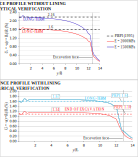
\includegraphics[scale = 1.0]{FIG6.pdf}
	\caption{\label{convergence_profile_piepi}Verification with Piepi (1995) analytical and numerical solution of the model elastoplastic-viscoplastic.}
\end{figure}

\section{Parametric analysis, results and discussions}

In this section, a parametric analysis is presented to investigate the influence of this elastoplastic-viscoplastic model on the long-term convergence profile, with and without lining. The rock mass properties are the same as the previous analysis with $E=1500$MPa. A variable lining modulus of $E_{rev} = 3000$MPa to $E_{rev} = 30000$MPa with $\nu_{rev} = 0.3$ and the unsupported distance of $d_0 = 0$ and $d_0 = 4L_p$ was adopted. Convergence at equilibrium is measured in $y/R_i = 6$. Fig.~\ref{convergence_lining_module} shows this results with elastic (E), viscoplastic (VP) and elastoplastic (EP) behavior. The stifness of the lining is calculated by the expression:
\begin{equation}
	\label{rigidez_revestimento}
	K_{rev} = \dfrac{E_{rev}}{(1+\nu_{rev})}\dfrac{R_i^2-(R_i-e_{rev})^2}{\left[(1-2\nu_{rev})R_i^2+(R_i-e_{rev})^2)\right]}.
\end{equation}


\begin{figure}
	\centering
	\includegraphics[scale = 1.0]{FIG7.pdf}
	\caption{\label{convergence_lining_module}Long-term convergence versus lining modulus of elasticity for an unsupported distance $d_0=0$ and $d_0=4L_p$.}
\end{figure}

When the lining stifiness is high, the model (VP) approaches the (EL). This is because the viscous deformations of the viscoplastic model are resisted by the lining and prevented to appear. In the other hand, the model (EPVP) approaches the model (EP). This is because during excavation and placement of the lining, some plastification occurs, but the viscous deformations of the model (EPVP) are resisted by the lining. Comparing the elastoplastic-viscoplastic  model with the viscoplastic model, in the long term, without lining, the (EPVP) had a 52\% higher convergence. With lining applied at $d_0=0$ a convergence of 23\% greater appears, and for $d_0=4L_p$ it is about 31\%. This is a big difference in relation to viscoplastic model that try to estimate the convergence in the long term, but do not consider the plastification of the rock mass in the instantaneous behavior.

The Fig.~\ref{unassociated_plasticity} shows the effect of using non-associative plastic flow on the convergence profile (at end of excavation and long-term) without lining. For the parameters used in the study, only a slight difference is observed between non-associated and associated plasticity. More parametric studies are needed to assess this particular aspect of the  constitutive behavior.

\begin{figure}
	\centering
	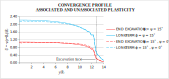
\includegraphics[scale = 1.0]{FIG8.pdf}
	\caption{\label{unassociated_plasticity}Comparison with associated and non-associated plasticity on the convergence profile (at end of excavation and long-term) without lining.}
\end{figure}

\section{Conclusions}

This work have presented a numerical integration scheme for the elastoplastic-viscoplastic constitutive behavior. A brief review of each model was performed separately and then their coupling. The numerical solution of the model was verified with the analytical and numerical solution obtained by \citeN {piepi1995} under axisymmetric conditions, demonstrating an excellent agreement. 

Finally, a parametric analysis was performed to show the importance of this model in the long-term convergence profile comparing with anotheres models that don't consider the instantaneous elastoplastic-viscoplastic behavior. For the considered properties, differences about of 23\% to 52\% were founded.

\section{Data Availability Statement}

Some or all data, models, or code that support the findings of this study are available from the corresponding author upon reasonable request. (ANSYS APDL script for FEM model and USERMAT subroutine in FORTRAN77 for constitutive rock mass model)

\pagebreak
%
% Now we start the Appendixes, with the new section name, "Appendix", and a 
%  new counter, "I", "II", etc.
%\appendix
%
%
% Now we start the appendices, with the new section name, "Appendix", and a 
%  new counter, "I", "II", etc.
%\appendix
%
% And now for some pretty impressive notation.  In this example, I have used
%   the tabular environment to line up the columns in ASCE style.
%   Note that this and all appendices (except the references) start with 
%   the \section command
%
%
% Here's the list of references:
%
% \label{section:references}
\bibliography{ascexmpl-new}
%

\end{document}
